\documentclass[11pt,twocolumn]{article}

\usepackage[T1]{fontenc}
\usepackage[utf8]{inputenc}
\usepackage{lmodern}
\usepackage[margin=0.75in]{geometry}
\usepackage{amsmath,amssymb,amsfonts}
\usepackage{graphicx}
\usepackage{booktabs}
\usepackage{array,tabularx}
\usepackage{hyperref}
\usepackage{xcolor}
\usepackage{microtype}
\usepackage[numbers,sort&compress]{natbib}
\usepackage{enumitem}
\usepackage{titlesec}
\setlist[enumerate]{leftmargin=*,itemsep=1pt,topsep=2pt}
\setlist[itemize]{leftmargin=*,itemsep=1pt,topsep=2pt}
\setlength{\parskip}{0pt}
\setlength{\parindent}{1em}
\titlespacing*{\paragraph}{0pt}{0.75\baselineskip}{0.5em}
\raggedbottom

\title{\textbf{Mask-Path InfoNCE without EMA in a\\
Global Image-Level JEPA: A CIFAR Study}}

\author{%
  Katakis Sofoklis\\
  \texttt{kat.sofoklis@gmail.com}
}

\date{}

\newcommand{\sg}{\mathrm{sg}}
\newcommand{\enc}{\mathrm{enc}}
\newcommand{\pred}{\mathrm{pred}}

\begin{document}
\maketitle

\begin{abstract}
Joint-Embedding Predictive Architectures (JEPAs) commonly stabilize latent
prediction with an exponential-moving-average (EMA) target encoder. We test
whether applying InfoNCE directly to the masked predictive pair can instead
train a single ResNet-18 encoder with stop-gradient targets and no EMA. Under a
matched 100-epoch CIFAR-10 protocol across three seeds, mask-path InfoNCE reaches
$42.6\mathbin{\pm}3.6\%$ $k$-nearest-neighbor accuracy and
$43.0\mathbin{\pm}3.4\%$ linear-probe accuracy, compared with
$41.6\mathbin{\pm}2.9\%$ and $41.3\mathbin{\pm}2.7\%$ for cosine JEPA with an
EMA target. The no-EMA method has slightly higher means, although the observed
variability does not establish a decisive advantage. These results support
mask-path contrast as a workable no-EMA option only in this restricted CIFAR
setting.
\end{abstract}
\section{Introduction}
\label{sec:intro}

Self-supervised learning (SSL) for visual representations spans two influential families:
\emph{contrastive} instance discrimination~\citep{chen2020simclr,he2020moco}
and \emph{predictive} joint embedding (JEPA)~\citep{assran2023ijepa,lecun2022path}.
I-JEPA predicts target-block embeddings from a context encoder and uses
regression in latent space with an EMA target network.
C-JEPA~\citep{mo2024cjepa} combines I-JEPA with variance--invariance--covariance
regularization (VICReg)~\citep{bardes2022vicreg} to stabilize training and improve
convergence on ImageNet.
These methods suggest several plausible substitutes for an EMA target: batch
negatives, variance--covariance constraints, or distribution matching.
However, a JEPA pipeline with both masked and augmented views introduces a
placement choice: the anti-collapse signal can act on masked prediction or on
a separate augmentation path.

We therefore ask: \emph{for a single-encoder JEPA without EMA, should contrast
act directly on masked prediction, or should masked prediction remain
non-contrastive while a separate augmentation path prevents collapse?} We
compare cosine mask$\rightarrow$clean prediction plus augmentation$\rightarrow$clean
InfoNCE with mask-path InfoNCE and non-contrastive augmentation regularizers.

\paragraph{Contributions.}
(i)~A controlled formulation that separates the masked predictive path from
the augmentation anti-collapse path;
(ii)~a matched CIFAR-10 comparison of contrastive, variance--covariance, and
Gaussian regularization with a single ResNet-18 encoder;
(iii)~evidence that mask-path InfoNCE is the strongest tested no-EMA objective,
while augmentation-side regularization does not improve on that baseline.

\section{Related work}
\label{sec:related}

\paragraph{Predictive JEPA.}
I-JEPA~\citep{assran2023ijepa} predicts latent targets under masking with
smooth-L1 / L2 and an EMA teacher, following the JEPA agenda of
LeCun~\citep{lecun2022path}.
\paragraph{C-JEPA.}
C-JEPA~\citep{mo2024cjepa} argues that EMA alone is insufficient to
prevent collapse and that mean-patch prediction is underconstrained; it
augments I-JEPA with VICReg~\citep{bardes2022vicreg} variance / covariance /
invariance terms and reports faster ImageNet convergence.
Our note shares C-JEPA's goal of combining predictive and contrastive-style
signals, but studies a much smaller CIFAR recipe: one encoder, stop-grad (no
EMA), cosine JEPA on the mask path, and either augmentation InfoNCE or a lightweight
regularizer (mean squared error with variance and covariance penalties, VICReg,
or Sketched Isotropic Gaussian Regularization (SIGReg)~\citep{balestriero2025lejepa}).

\paragraph{Contrastive and non-contrastive SSL.}
SimCLR~\citep{chen2020simclr} and MoCo~\citep{he2020moco} use InfoNCE on two
augmented views.
BYOL~\citep{grill2020byol} and SimSiam~\citep{chen2021simsiam} avoid
explicit negatives via predictors and stop-grad / EMA.
Barlow Twins~\citep{zbontar2021barlow} and VICReg~\citep{bardes2022vicreg}
prevent collapse with redundancy-reduction / variance--covariance penalties
rather than negatives.

\begin{table*}[t]
  \centering
  \small
  \setlength{\tabcolsep}{6pt}
  \caption{CIFAR-10, ResNet-18, evaluated at the fixed 100-epoch endpoint.
  Learned-model results are mean $\mathbin{\pm}$ sample standard deviation over seeds 42, 7, and 123.
  Random chance is included as a reference baseline.
  Cosine JEPA $+$ augmentation InfoNCE places batch negatives only on the augmentation path.
  Hybrids $=$ cosine JEPA (mask) $+$ listed augmentation/clean regularizer (no EMA).
  All reported runs are complete.}
  \label{tab:cifar10}
  \begin{tabularx}{\textwidth}{>{\raggedright\arraybackslash}Xccc}
    \toprule
    Method & $k$-NN & Linear & Seeds \\
    \midrule
    \multicolumn{4}{l}{\emph{Reference baselines}} \\
    Random classifier (chance)
      & 0.100 & 0.100 & -- \\
    Supervised CE
      & $0.949 \pm 0.001$ & $0.948 \pm 0.001$ & 3 \\
    \midrule
    \multicolumn{4}{l}{\emph{Self-supervised learning}} \\
    EMA JEPA cosine
      & $0.416 \pm 0.029$ & $0.413 \pm 0.027$ & 3 \\
    JEPA InfoNCE (mask only; no EMA)
      & $\mathbf{0.426 \pm 0.036}$ & $\mathbf{0.430 \pm 0.034}$ & 3 \\
    Cosine JEPA $+$ augmentation InfoNCE (no EMA)
      & $0.402 \pm 0.010$ & $0.399 \pm 0.019$ & 3 \\
    JEPA $+$ MSE/variance/covariance (no EMA)
      & $0.397 \pm 0.002$ & $0.346 \pm 0.063$ & 3 \\
    JEPA $+$ VICReg (no EMA; $25$/$25$/$25$)
      & $0.374 \pm 0.004$ & $0.393 \pm 0.007$ & 3 \\
    JEPA $+$ SIGReg (no EMA)
      & $0.383 \pm 0.008$ & $0.407 \pm 0.004$ & 3 \\
    \bottomrule
  \end{tabularx}
\end{table*}

\begin{table*}[t]
  \centering
  \small
  \setlength{\tabcolsep}{8pt}
  \caption{CIFAR-100, ResNet-18, seed 42, evaluated at the fixed 100-epoch endpoint.
  These exploratory single-seed results are reported separately from the
  three-seed CIFAR-10 comparison and do not include uncertainty estimates.}
  \label{tab:cifar100}
  \begin{tabularx}{\textwidth}{>{\raggedright\arraybackslash}Xccc}
    \toprule
    Method & $k$-NN & Linear & Epoch \\
    \midrule
    Random classifier (chance)
      & 0.010 & 0.010 & -- \\
    EMA JEPA cosine
      & 0.125 & 0.129 & 100 \\
    JEPA InfoNCE (mask only; no EMA)
      & \textbf{0.155} & \textbf{0.150} & 100 \\
    Cosine JEPA $+$ augmentation InfoNCE (no EMA)
      & 0.118 & 0.106 & 100 \\
    \bottomrule
  \end{tabularx}
\end{table*}

\begin{figure*}[t]
  \centering
  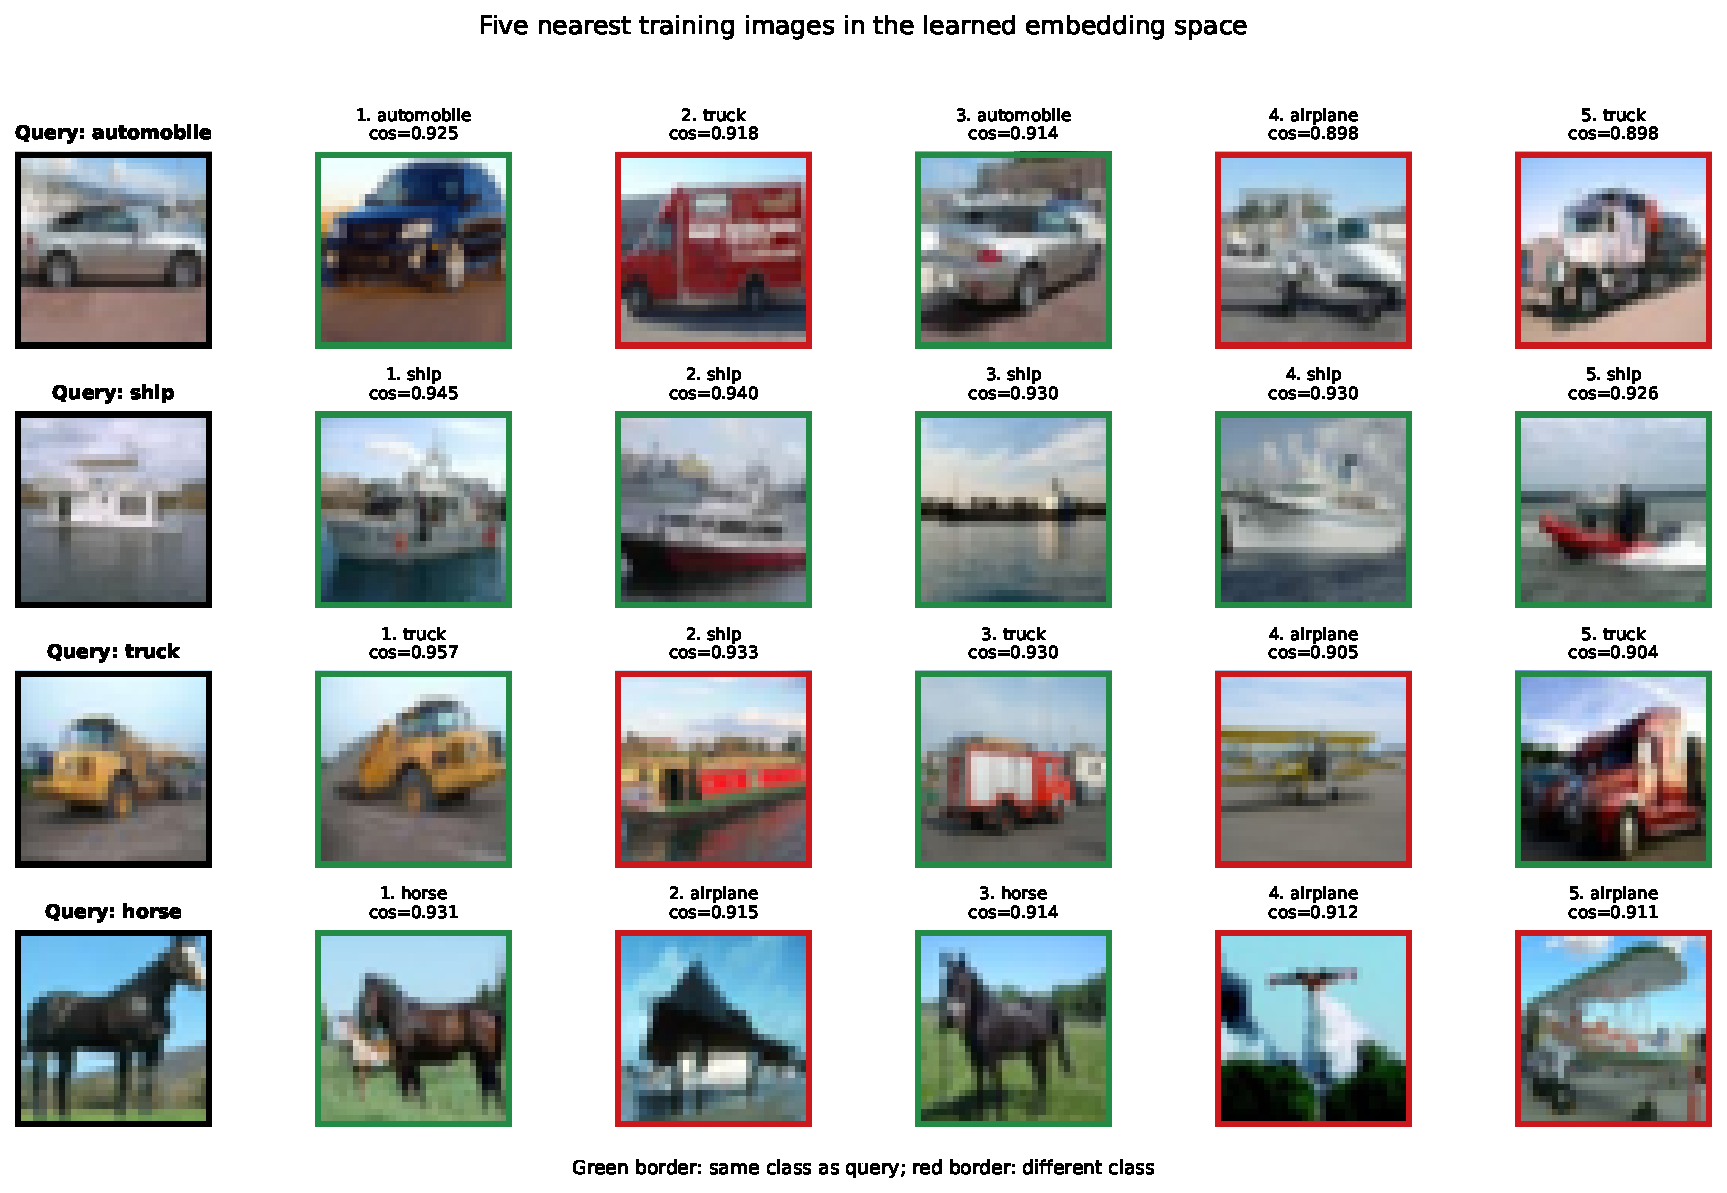
\includegraphics[width=0.84\textwidth]{figures/nearest_neighbors_mask_infonce.pdf}
  \caption{Five nearest training images for four test queries under cosine
  similarity in the frozen mask-only InfoNCE representation. The encoder is
  the best checkpoint at epoch 80. The four representative queries span
  automobile, ship, truck, and horse; their fixed test indices are provided
  with the figure metadata. Retrieval uses all 50,000 training images with
  deterministic evaluation preprocessing. Green borders indicate the query
  class and red borders a different class. The examples expose both coherent
  neighborhoods and cross-class confusion, consistent with the moderate
  aggregate $k$-NN accuracy.}
  \label{fig:nearest-neighbors}
\end{figure*}

\section{Methods and Objectives}
\label{sec:method}

\paragraph{Views and notation.}
For each image $x$, we form a lightly augmented clean view $x_c$, a
block-masked view $x_m$, and a strongly augmented view $x_a$. A single encoder
$f_\theta$ maps each view to a 512-dimensional representation, and a predictor
$g_\phi$ is used only on the masked path:
\begin{equation}
 z_c=f_\theta(x_c),\qquad
 \hat z_m=g_\phi(f_\theta(x_m)),\qquad
 z_a=f_\theta(x_a).
 \label{eq:representations}
\end{equation}
The predictor is discarded at evaluation. Except for the EMA reference, all
objectives use the same online encoder. The notation $\sg(\cdot)$ denotes
stop-gradient. It is applied to the clean target in the cosine and InfoNCE
predictive pairs, but not between the two branches of the variance--covariance
or SIGReg augmentation regularizers.

\paragraph{Cosine JEPA.}
The non-contrastive masked-prediction objective is
\begin{equation}
 L_{\mathrm{cos}}=1-\frac{\hat z_m^\top\sg(z_c)}
 {\|\hat z_m\|_2\,\|\sg(z_c)\|_2}.
 \label{eq:jepa}
\end{equation}
Averaging over the batch is implicit. This objective enforces invariance
between masked and clean views but contains no explicit term requiring
features from different images to remain distinct. Consequently, a
single-encoder version can admit collapsed or weak representations. The EMA
baseline uses the same cosine loss but computes the clean target with a
momentum encoder $f_\xi$, updated as
$\xi\leftarrow m\xi+(1-m)\theta$ with $m=0.996$.

\paragraph{InfoNCE.}
For query--key pairs $q_i,k_i$ in a batch of size $B$, we use
\begin{equation}
 L_{\mathrm{NCE}}(q,k)=-\frac{1}{B}\sum_{i=1}^{B}\log
 \frac{\exp(\bar q_i^\top\bar k_i/\tau)}
 {\sum_{j=1}^{B}\exp(\bar q_i^\top\bar k_j/\tau)},
 \label{eq:nce}
\end{equation}
where bars denote $\ell_2$ normalization and $\tau=0.1$. The matching view of
the same image is the positive; the other $B-1$ clean embeddings are
negatives. Stop-gradient is applied to every key. We compare two placements:
\begin{align}
 L_{\mathrm{mask\text{-}NCE}}
   &=L_{\mathrm{NCE}}(\hat z_m,\sg(z_c)), \\
 L_{\mathrm{cos+aug\text{-}NCE}}
   &=L_{\mathrm{cos}}+L_{\mathrm{NCE}}(z_a,\sg(z_c)).
 \label{eq:placements}
\end{align}
Thus, mask-only InfoNCE makes the predictive task itself contrastive, whereas
the second objective preserves non-contrastive masked prediction and places
instance discrimination only on the augmentation path. Both active terms have
unit weight.

\paragraph{MSE, variance, and covariance.}
To test negative-free anti-collapse regularization, we replace augmentation
InfoNCE with the three VICReg building blocks. For $z\in\mathbb{R}^{B\times D}$,
\begin{align}
 L_{\mathrm{inv}}&=\frac{1}{BD}\|z_a-z_c\|_F^2,\\
 v(z)&=\frac{1}{D}\sum_{d=1}^{D}
 \max\!\left(0,1-\sqrt{\operatorname{Var}(z_{:,d})+\epsilon}\right),\\
 c(z)&=\frac{1}{D}\sum_{r\ne s}\operatorname{Cov}(z)_{rs}^{2},
 \label{eq:vicreg-components}
\end{align}
with $\epsilon=10^{-4}$. The invariance term aligns the two views, the variance
hinge prevents individual dimensions from becoming constant, and the
covariance penalty discourages redundant dimensions. The complete objective is
\begin{align}
 L_{\mathrm{MVC}}={}&L_{\mathrm{cos}}+\lambda_iL_{\mathrm{inv}}
 +\lambda_v[v(z_a)+v(z_c)] \notag\\
 &+\lambda_c[c(z_a)+c(z_c)].
 \label{eq:mvc}
\end{align}
We evaluate unit weights $(\lambda_i,\lambda_v,\lambda_c)=(1,1,1)$ and the
VICReg-scale setting $(25,25,25)$ reported as separate rows. Gradients flow
through both $z_a$ and $z_c$ in these three terms.

\paragraph{SIGReg.}
Sketched Isotropic Gaussian Regularization (SIGReg) replaces the explicit
variance and covariance penalties with a distribution-matching term. We
concatenate both augmentation branches, $Z=[z_a;z_c]$, project $Z$ onto 256
deterministically seeded random unit directions, and compare each projected
empirical characteristic function with that of $\mathcal{N}(0,1)$ using the
Epps--Pulley statistic~\citep{balestriero2025lejepa}. In compact form,
\begin{align}
 L_{\mathrm{SIG}}={}&L_{\mathrm{cos}}+L_{\mathrm{inv}} \notag\\
 &+\frac{1}{R}\sum_{r=1}^{R}
 \mathcal{E}(Z u_r,\mathcal{N}(0,1)),\quad R=256,
 \label{eq:sigreg}
\end{align}
where $u_r$ is a random unit direction and $\mathcal{E}$ is the weighted
characteristic-function discrepancy. All three terms use unit weight. SIGReg
encourages a non-degenerate, approximately isotropic latent distribution while
$L_{\mathrm{inv}}$ preserves augmentation invariance.

\paragraph{Controlled comparison.}
Across the no-EMA rows, the encoder, predictor, views, optimizer, and training
budget are fixed; only the objective and its stated weights change. This
separation lets us test whether anti-collapse behavior depends not only on the
regularizer family but also on the path to which it is applied.





\section{Experimental protocol}
\label{sec:protocol}

\paragraph{Data and architecture.}
CIFAR-10~\citep{krizhevsky2009cifar}; ResNet-18~\citep{he2016resnet}
with embedding dimension $512$; a predictor multilayer perceptron (MLP) on the mask path.
Block masking with mask ratio $0.6$.
Strong augs: random resized crop, horizontal flip, color jitter
($B{=}C{=}S{=}0.4$, hue $0.1$).

\paragraph{Optimization.}
Adam, learning rate $3{\times}10^{-4}$, batch size $256$, $100$ epochs,
InfoNCE temperature $\tau{=}0.1$, one encoder (no EMA).

\paragraph{Evaluation.}
Frozen encoder; $k$-NN ($k{=}20$) and linear probe (standard CIFAR split).
Evaluate every 10 epochs and select the checkpoint with best $k$-NN.

\paragraph{Hardware and runtime.}
Experiments were run on NVIDIA GeForce RTX 5060 Ti GPUs (16~GB), using one GPU
per run. Including periodic frozen-feature evaluation, the 100-epoch mask-only
InfoNCE run took 11,721~s (3.26~h), while cosine JEPA plus augmentation InfoNCE
took 10,546~s (2.93~h). The two runs can be executed concurrently on two GPUs,
for approximately 3.26~h wall-clock time.

\paragraph{Baselines (same stack).}
\begin{itemize}
  \item Supervised cross-entropy (CE; upper bound);
  \item EMA JEPA cosine (teacher EMA);
  \item JEPA InfoNCE on the mask path only (no augmentation term);
  \item Cosine JEPA $+$ augmentation InfoNCE;
  \item Hybrids: cosine JEPA (mask$\rightarrow$clean, no EMA) $+$ MSE/variance/covariance,
        SIGReg~\citep{balestriero2025lejepa}, or
        VICReg~\citep{bardes2022vicreg} on augmentation/clean;
\end{itemize}





\section{Results}
\label{sec:results}

All numbers below are CIFAR-10, ResNet-18 ($D{=}512$), batch $256$, $100$ epochs,
frozen $k$-NN ($k{=}20$) and linear probe. We report the fixed epoch-100
endpoint as mean $\mathbin{\pm}$ sample standard deviation over three seeds
(42, 7, and 123) for both supervised and self-supervised models.





\paragraph{Qualitative neighborhoods.}
Figure~\ref{fig:nearest-neighbors} shows the five most similar training images
for fixed test queries spanning four classes. The class-consistent ship
neighborhood contrasts with mixed automobile, truck, and horse neighborhoods.
This qualitative variation helps explain why local similarity is useful but
far from class-perfect.

\paragraph{Mask-path contrast is strongest.}
Mask-only InfoNCE is the best tested SSL method by both $k$-NN
($0.426\mathbin{\pm}0.036$) and linear probe ($0.430\mathbin{\pm}0.034$).
It exceeds the EMA cosine-JEPA reference by about one percentage point on each
mean while using no teacher encoder. This suggests that batch negatives on the
predictive pair can supply an effective anti-collapse signal in the present
regime, although the overlapping uncertainty cautions against claiming a
decisive advantage over EMA.

\paragraph{Augmentation-side contrast is not an equivalent substitute.}
Cosine JEPA plus augmentation InfoNCE reaches
$0.402\mathbin{\pm}0.010$ $k$-NN and $0.399\mathbin{\pm}0.019$ linear accuracy,
trailing mask-only InfoNCE on both means. Its smaller variance does not recover
the average representation quality, supporting the view that contrast placement matters.

\paragraph{Distributional regularizers trail mask-path contrast.}
The cosine-JEPA regularizers do not recover the mask-only InfoNCE result.
MSE/variance/covariance has stable $k$-NN ($0.397\mathbin{\pm}0.002$) but a
variable linear probe ($0.346\mathbin{\pm}0.063$). VICReg reaches
$0.374\mathbin{\pm}0.004$/$0.393\mathbin{\pm}0.007$, while SIGReg reaches
$0.383\mathbin{\pm}0.008$/$0.407\mathbin{\pm}0.004$ ($k$-NN/linear).
The mismatch between neighborhood and linear metrics cautions against ranking
representations with only one evaluator.

\section{Discussion and limitations}
\label{sec:discussion}

\paragraph{Relation to C-JEPA.}
C-JEPA~\citep{mo2024cjepa} combines I-JEPA with VICReg on large-scale ImageNet
pretraining and retains an EMA teacher.
We target a minimal CIFAR recipe without EMA: cosine JEPA on the mask path for
``ours'' and for the regularizer hybrids
(MSE/variance/covariance, SIGReg~\citep{balestriero2025lejepa},
VICReg~\citep{bardes2022vicreg}).

\paragraph{Limitations.}
CIFAR-10, ResNet-18, and three seeds are insufficient for broad claims about
JEPA training, and the objectives were not tuned with equal hyperparameter
budgets. We lack a matched augmentation-InfoNCE-only control and ImageNet-scale
validation. Although fixed-epoch reporting avoids selecting the endpoint by
test $k$-NN, hyperparameter development still used the same benchmark; future
experiments should use a held-out validation split. Finally, our global
image-level target simplifies I-JEPA's block-level prediction task.

\paragraph{Takeaway.}
A single encoder can learn non-collapsed masked representations without EMA,
but the successful ingredient is not merely the presence of an anti-collapse
loss. At epoch 100, mask-path InfoNCE is the strongest tested choice on average
($0.426\mathbin{\pm}0.036$ $k$-NN, $0.430\mathbin{\pm}0.034$ linear); cosine
prediction paired with augmentation-side InfoNCE or distributional
regularization is weaker under the evaluated settings. The practical lesson is
to treat loss placement as a first-class design choice in predictive--contrastive SSL.

\bibliographystyle{plainnat}
\bibliography{references}

\end{document}
